\documentclass{article}
\usepackage{graphicx}
\usepackage[utf8]{inputenc}
\usepackage{multicol}

\title{WEB ARCHITECTURES \\Assignment 4}
\author{Riccardo Gennaro}
\date{\today}

\begin{document}

\maketitle

\section{Introduction}

\subsection*{Problem statement}

This project aims at developing a simple web application capable of displaying to a user information about a given student. In particular, there are two use case: the request for student info, that displays anagraphics and choosen courses, and the advisor choice, that displays the anagraphics of a given student and the teachers of the courses he/she is enrolled in.

As requested by the assignment, the business logic must be implemented through EJB and deployed on a WildFly server that lays outside of the Tomcat were the client side must reside.

\section{Proposed solution}

This assignment is divided in two projects, one deployed on WildFly, one on Tomcat.

\subsection*{Tomcat - Servlets}

\subsubsection*{HomeServlet}

It is the welcome file, and it simply presents the \texttt{index.jsp} from which it is possible to input (through a form) the student ID for requesting the student info or to access the advisor choice. Using a non-registered student ID will display an error message.

\subsubsection*{StudentServlet}

This servlet makes use of the \texttt{StudentManagerBD} to access the data of a given student and displays it through \texttt{studentPage.jsp}.
The requested data are:
\begin{itemize}
    \item Student name;
    \item Student surname;
    \item Student ID;
    \item Courses in which the student is enrolled;
    \item Grades of the above courses, if any.
\end{itemize}

\subsubsection*{StudentServlet}

This servlet makes use of the \texttt{AdvisorChoiceBD} to access the data of a given student and displays it through \texttt{advisorChoice.jsp}.
The requested data are:
\begin{itemize}
    \item Student name;
    \item Student surname;
    \item Student ID;
    \item Names of the teachers that theac the courses in which the student is enrolled;
\end{itemize}

\subsection*{Tomcat - Business Delegates}

Both classes \texttt{AdvisorChoiceBD} and \texttt{StudentManagerBD}, are used to access facade \texttt{AdvisorChoiceManagerFacade} and facade \texttt{StudentManagerFacade} functions. To do so, the business delegates instantiate these interfaces through the Service Locator.

\subsection*{Tomcat - Service Locator}

\subsubsection*{RemoteServiceInitializer}

This class is a singleton used to set the JNDI properties and to operate the lookup in order to make accessible the services that resides in the WildFly server. It also implements a caching of the already looked up services. The caching is implemented through the \texttt{cache} hashmap;

\subsection*{WildFly - Facade Beans}

As anticipated above, this solution impents two facade. This facades implementations are two beans that expose their methods to execute high-level operations. To do so,  
To answer the client, this beans converts the entity to a detatched version of the object, a DTO. To build the DTO, class \texttt{DTOAssembler} is used.

\subsection*{WildFly - Entity Beans}

This beans are not exposed to the client, but are used in order to interact with the entities through the \texttt{EntityManager} class. This beans implement the communication with the database. This beans are accessed by the facade implementation through injection operated by the @EJB annotation used in the facade bean.

\subsection*{Database and entities}

Following the database ER-schema.

\begin{figure}[h!]
    \centering
    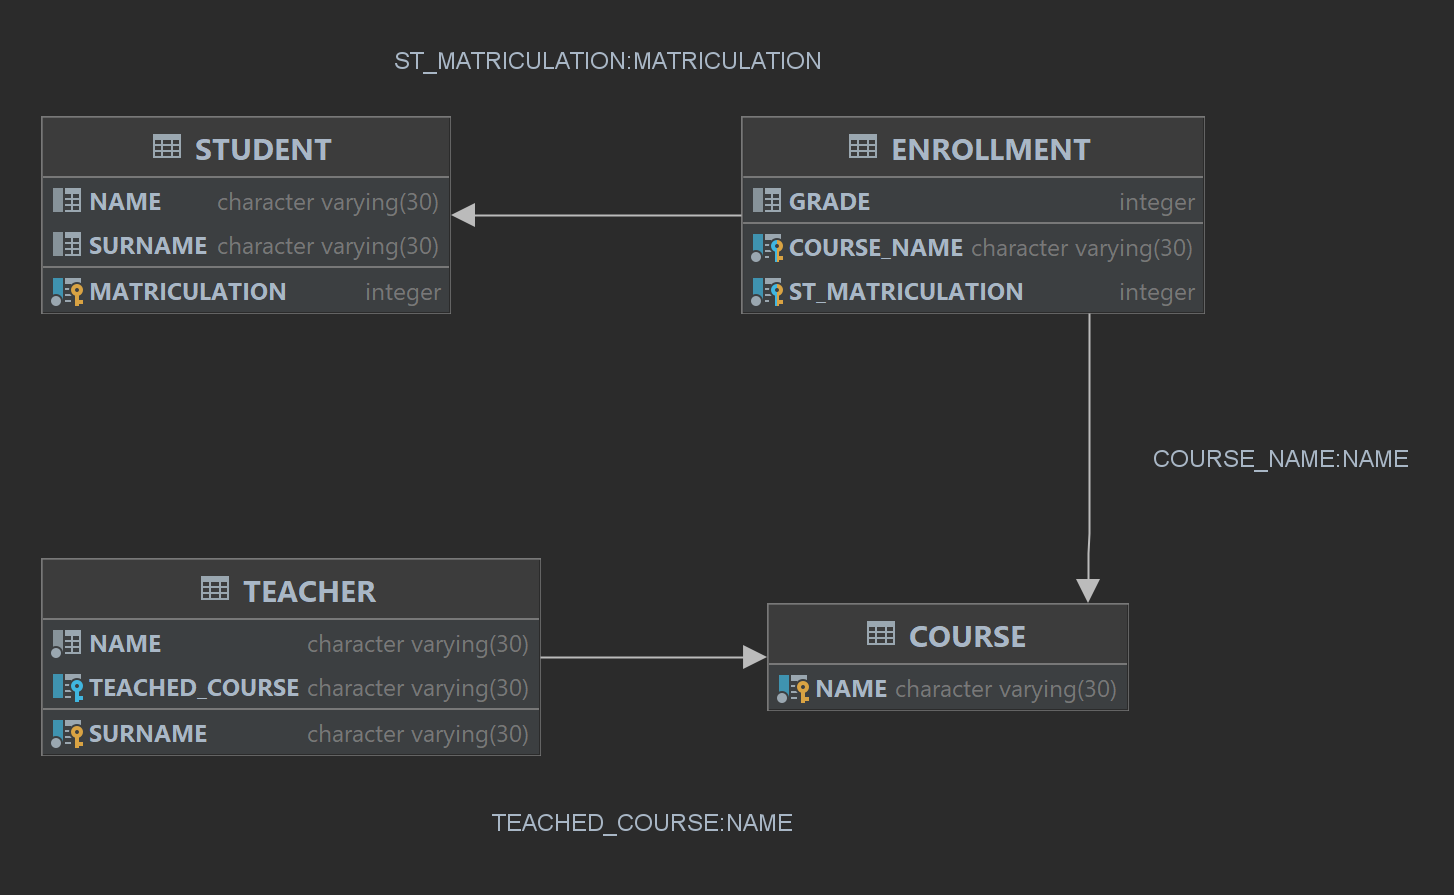
\includegraphics[keepaspectratio,width=1\textwidth]{drawable/Assignment4_ER.png}
    \caption{Database ER}
\end{figure}

There are four tables

\begin{itemize}
    \item STUDENT, with three columns:
    \begin{itemize}
        \item NAME
        \item SURNAME
        \item MATRICULATION (Primary Key)
    \end{itemize}
    \item TEACHER, with three columns
    \begin{itemize}
        \item NAME
        \item SURNAME (Primary Key)
        \item TEACHED\textunderscore COURSE (Foreign Key, for 1:1 relation with table COURSE)
    \end{itemize}
    \item COURSE, with a single column
    \begin{itemize}
        \item NAME
    \end{itemize}
    \item ENROLLMENT, table used to implement the N:M relation between tables STUDENT and COURSE.
    \begin{itemize}
        \item GRADE
        \item COURSE\textunderscore NAME
        \item ST \textunderscoreMATRICULATION
    \end{itemize}
    ENROLLMENT primary key is given by pair (COURSE\textunderscore NAME, ST\textunderscore MATRICULATION).
\end{itemize}

To connect the database the file \texttt{resources/META-INF/persistence.xml} has been modified to include tag \texttt{<jta-data-source> java:jboss/datasources/mydb </jta-data-source>}. The datasource has been configured via WildFly's \texttt{standalone.xml}. The edited \texttt{datasource} tag of the \texttt{standalone.xml} can be found at the base path of this deliverable in file \texttt{standaloneSnippet.xml}.
The database data have been exported through files \texttt{mydb.mv.db} and \texttt{mydb.trace.db} and can be found at the base path of this deliverable.

\newpage

\section*{Running application}

\subsection*{Welcome Page}

\begin{figure}[h!]
    \centering
    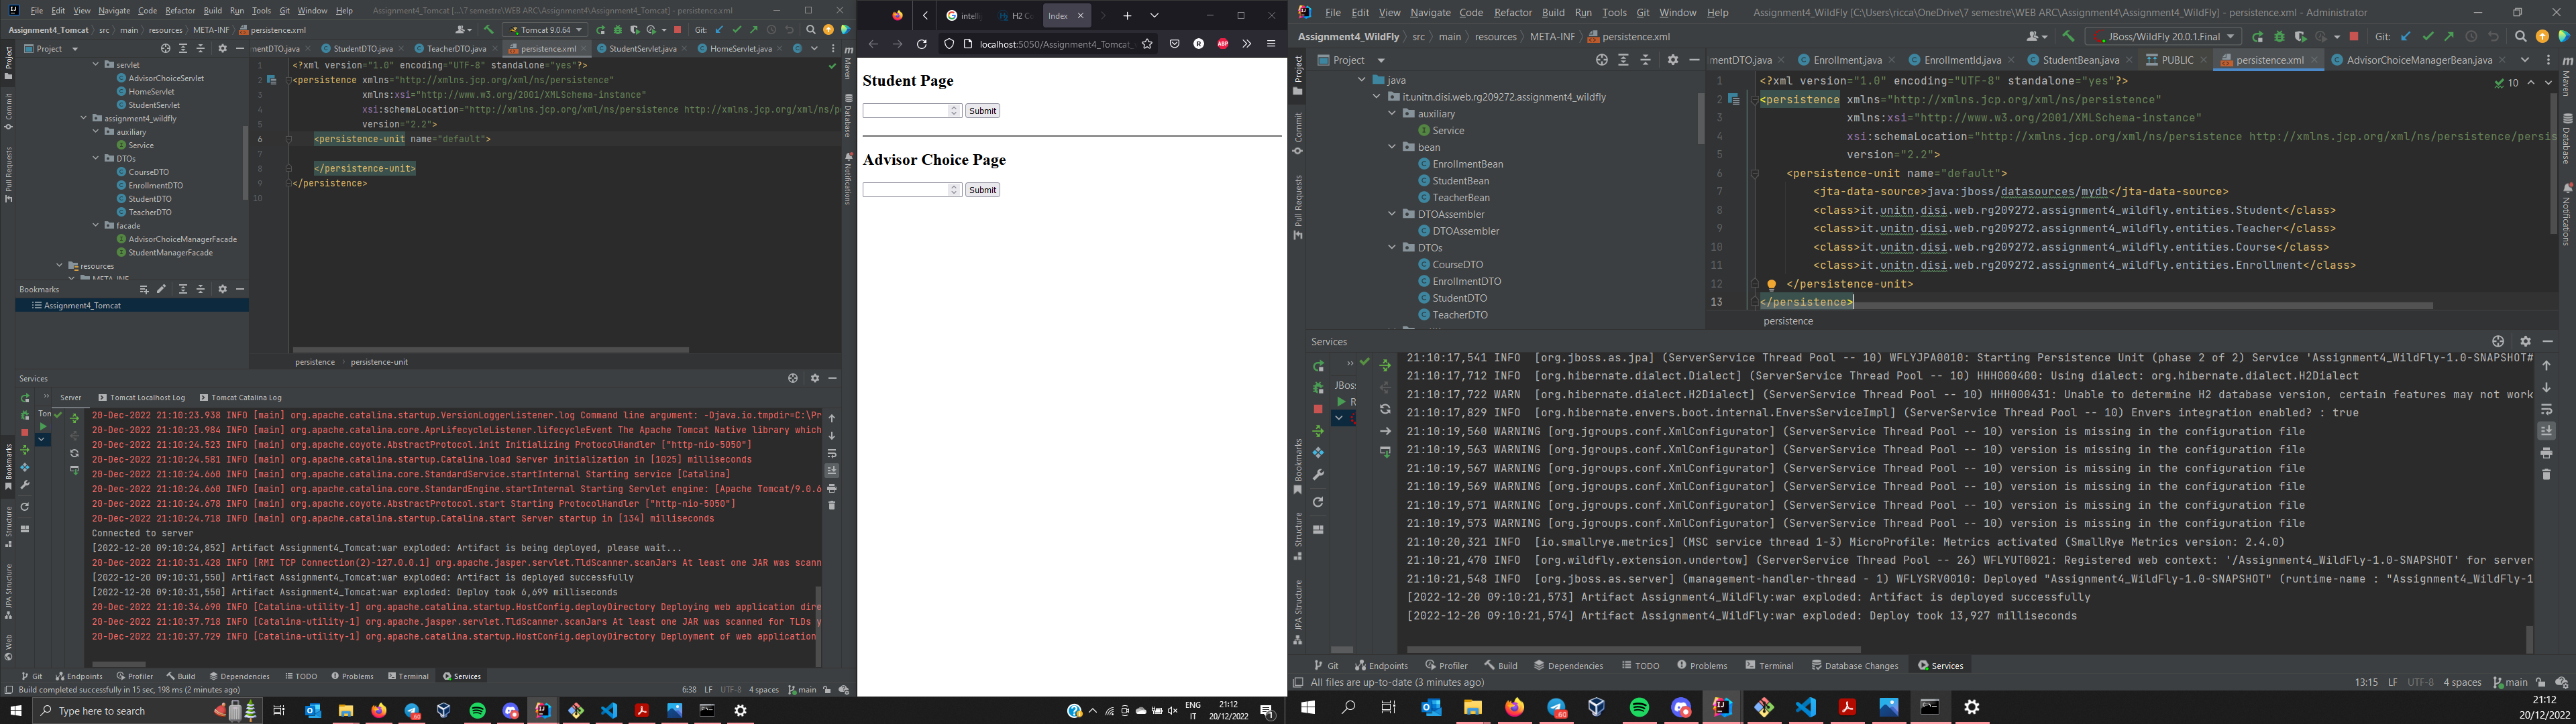
\includegraphics[keepaspectratio,width=1\textwidth]{drawable/welcomePage.PNG}
    \caption{Initial page. There are two forms: one redirects to Student Info, the other to the Advisor Choice}
\end{figure}

\begin{figure}[h!]
    \centering
    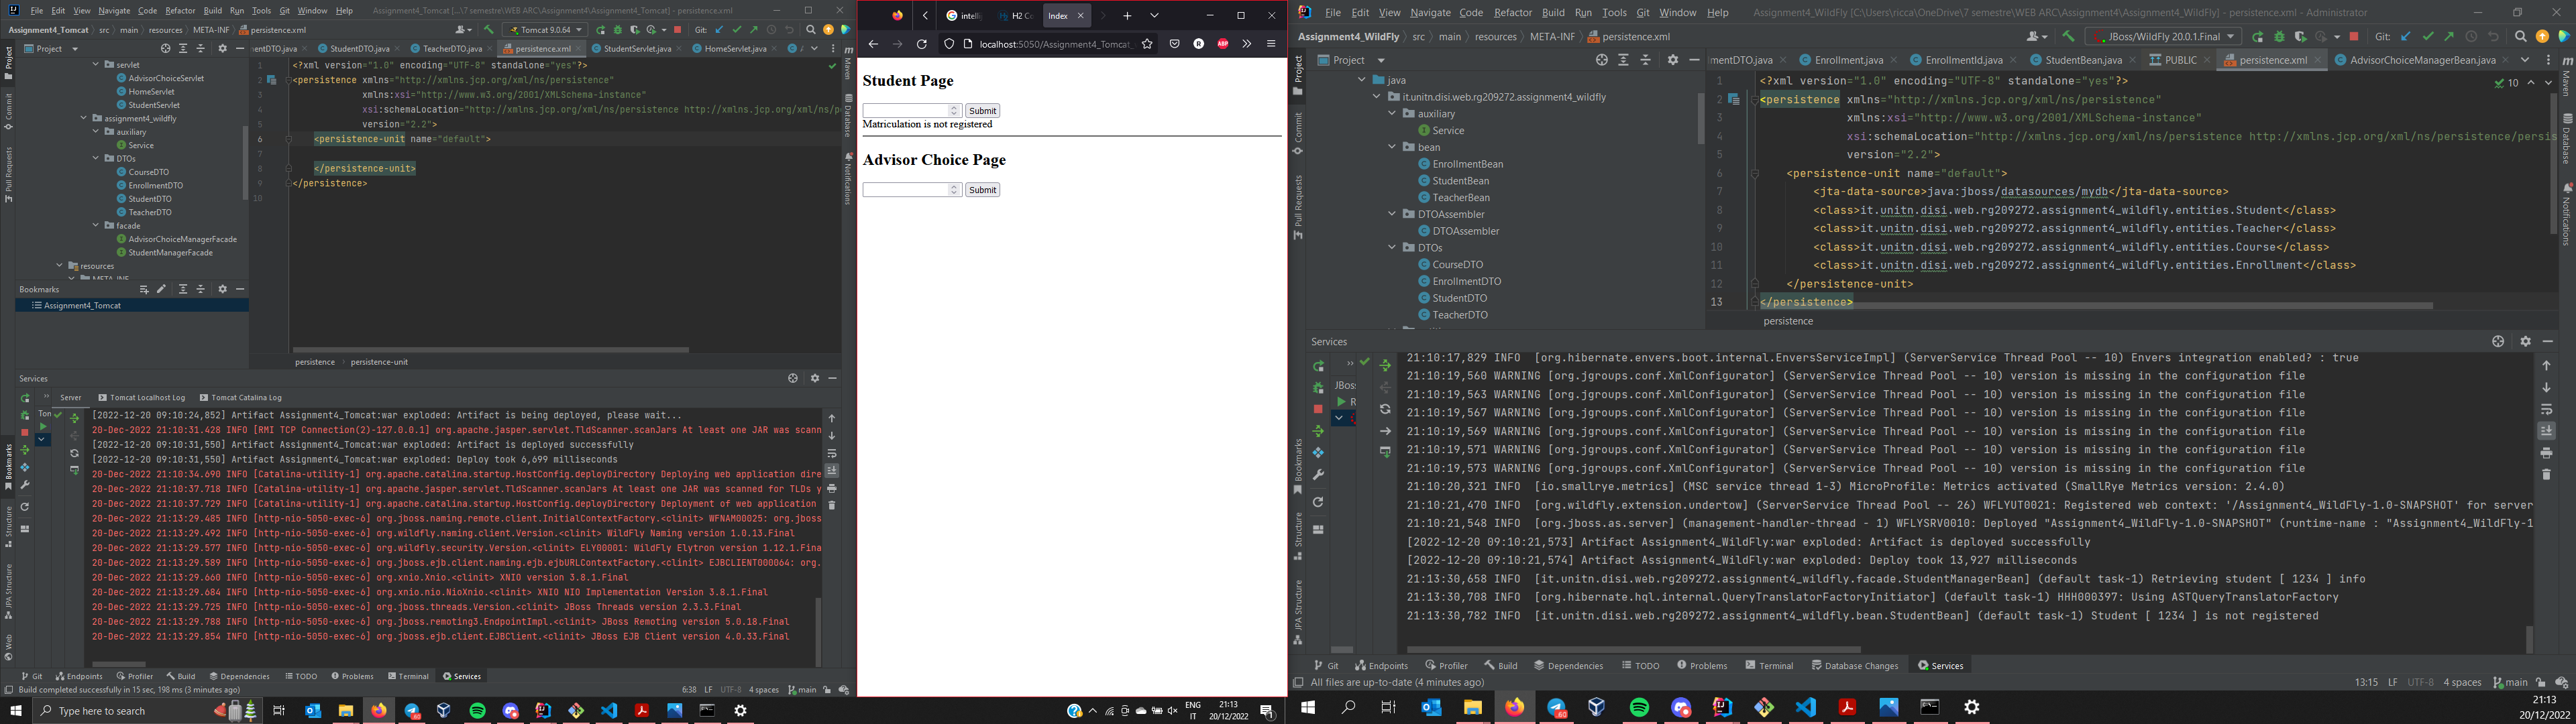
\includegraphics[keepaspectratio,width=1\textwidth]{drawable/MatriculationDoNotExist.PNG}
    \caption{Initial page. A non-registered student ID was requested}
\end{figure}

\begin{figure}[h!]
    \centering
    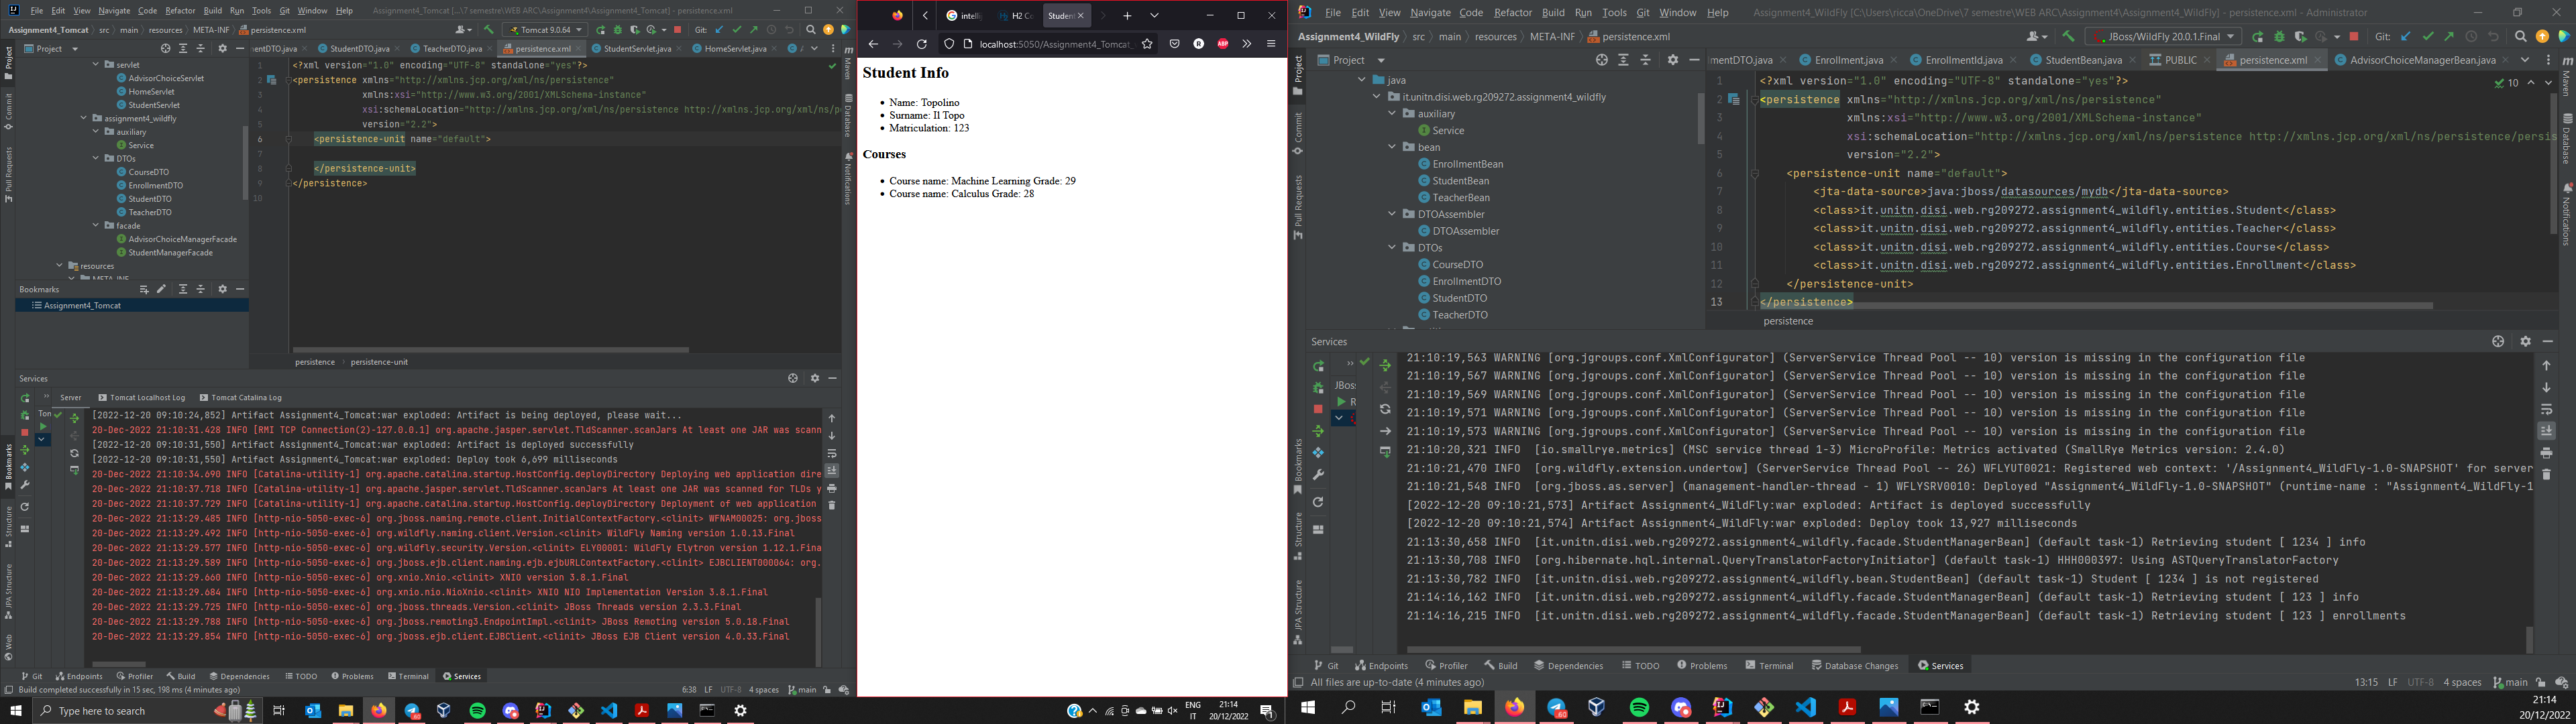
\includegraphics[keepaspectratio,width=1\textwidth]{drawable/Test123.PNG}
    \caption{Student page.}
\end{figure}

\begin{figure}[h!]
    \centering
    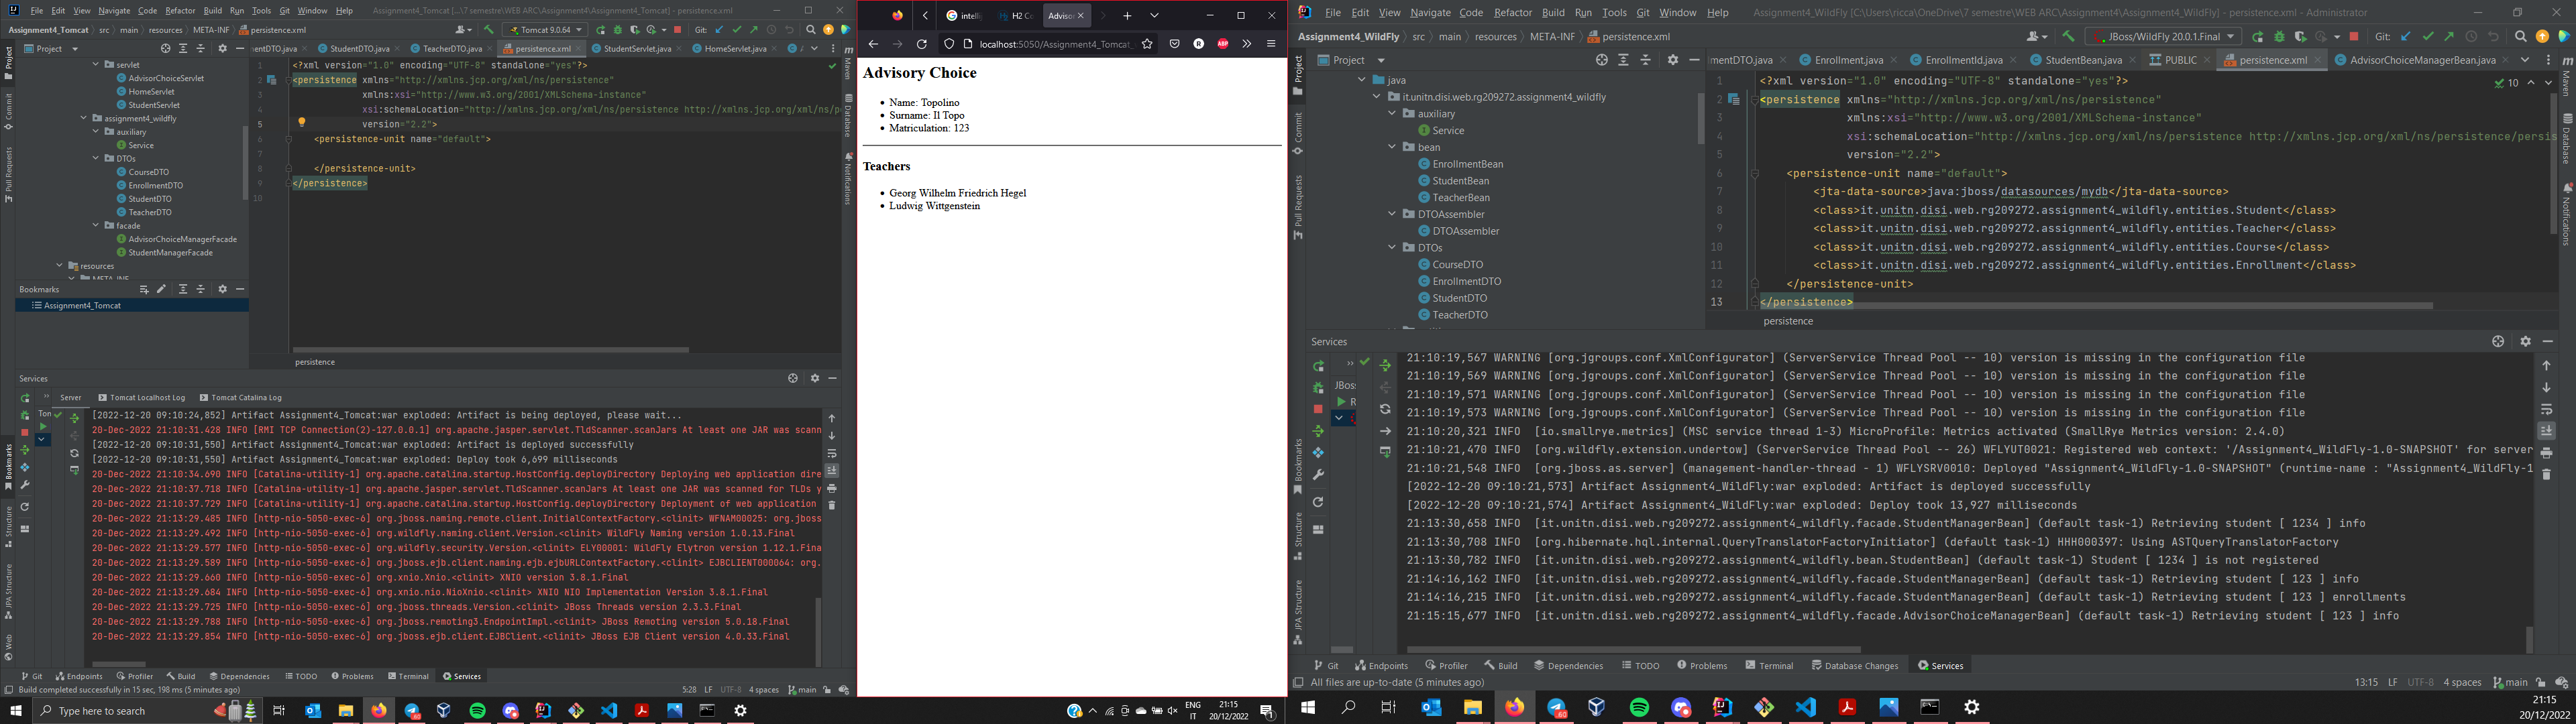
\includegraphics[keepaspectratio,width=1\textwidth]{drawable/TestAdvisor123.PNG}
    \caption{Advisor Choice page}
\end{figure}

\begin{figure}[h!]
    \centering
    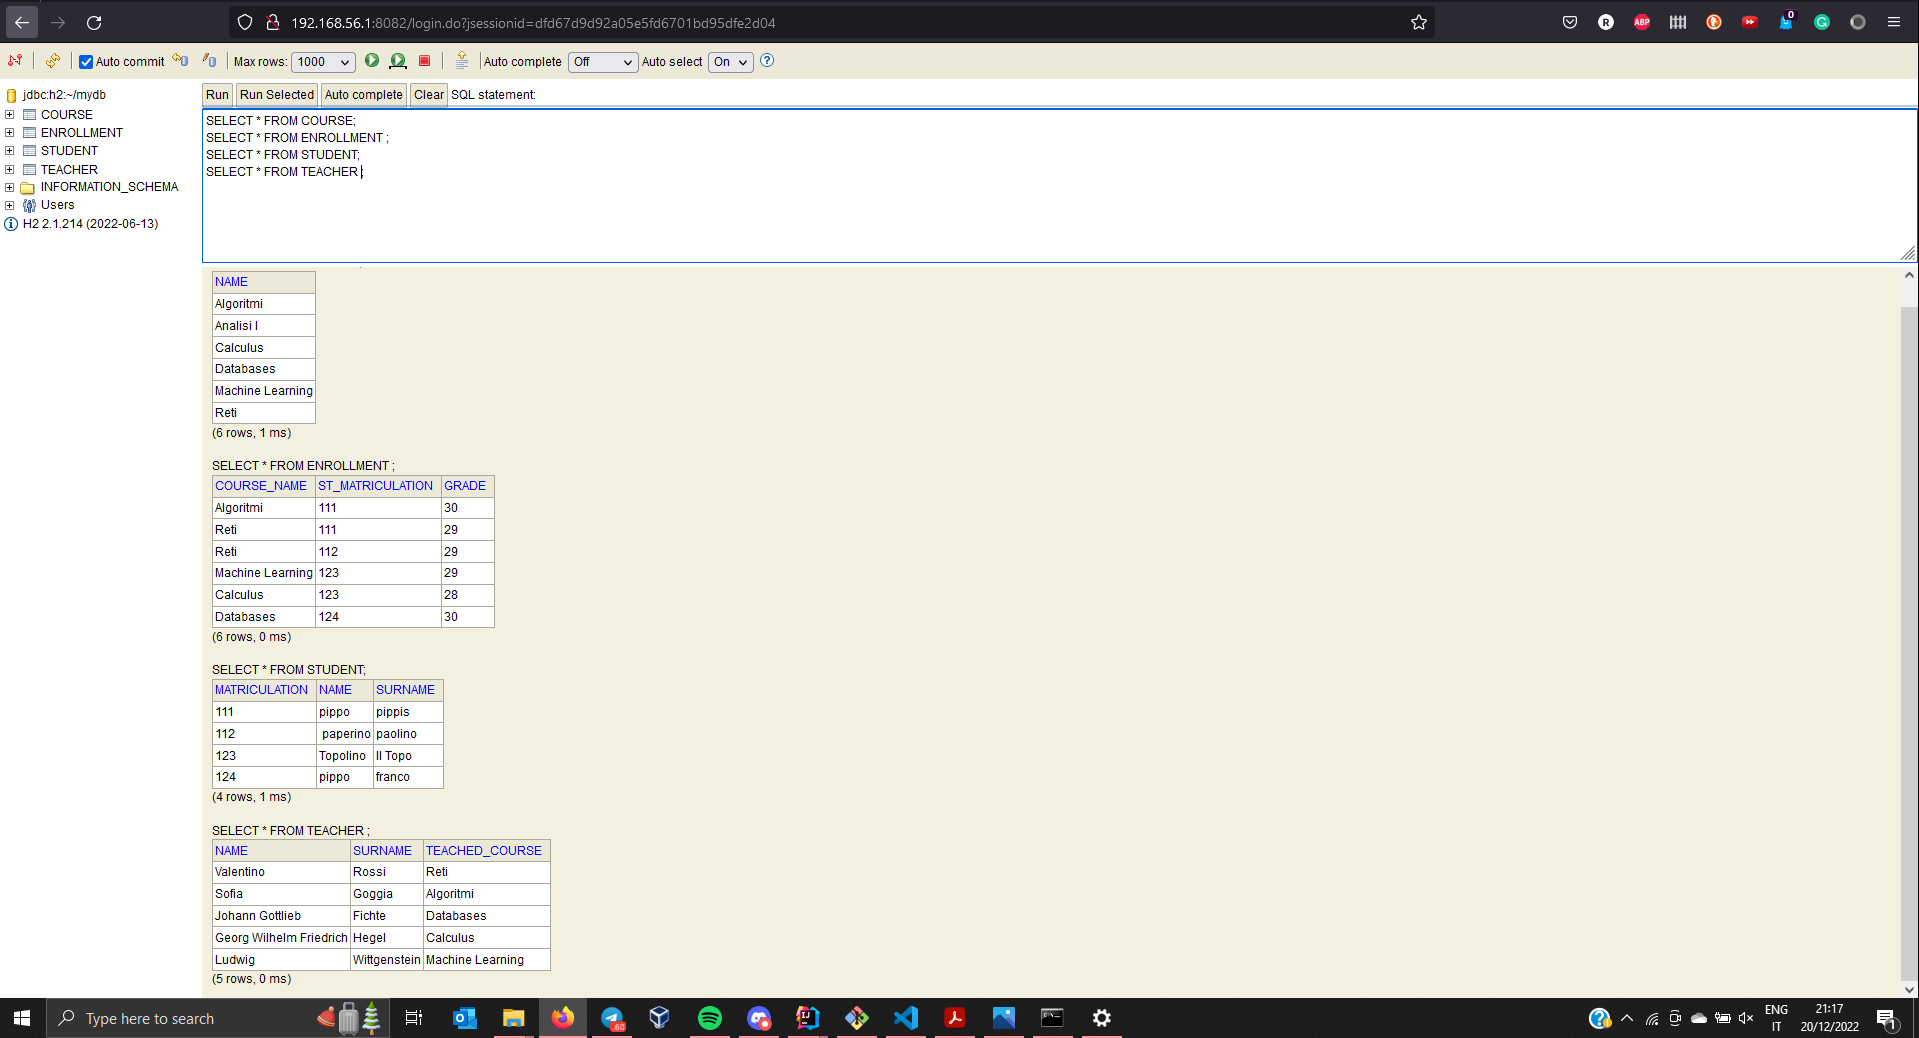
\includegraphics[keepaspectratio,width=1\textwidth]{drawable/db.PNG}
    \caption{Database Tables}
\end{figure}

\newpage

\section*{Comments and notes}

The project presents duplicated code. In particular, packages \\\texttt{it.unitn.disi.web.rg209272.assignment4\textunderscore wildfly.auxiliary | DTOs | facade} are duplicated both in Tomcat and WildFly sides. A solution could be including this packages through maven dependencies. I tried doing so, but WildFly threw a bunch of errors about the name of the service and I didn't have time to investigate.

Also, I must say that one of the biggest challenges was the configuration of WildFly and the understanding of the requested patterns.

\end{document}